%\chapter{Movimientos}
\label{chapter:busqueda}
\section{Busqueda y Pateo}


\subsection{Movimiento del esqueleto}

El robot debe desplazarse para poder patear la pelota por ello se describen y definen los movimientos del esqueleto que se fueron utilizados.

Con fines explicativos, en este proyecto, la palabra ''pose" se referire a la posición específica de los 16 motores que constituyen el esqueleto del robot. Un conjunto de poses ejecutadas en secuencia se denominará ''acción de movimiento".


Las acciones de movimiento establecidas son:


\begin{itemize}
 \item {Caminar hacia adelante}
 \item {Girar a la izquierda}
 \item {Girar a la derecha}
 \item {Levantarse cuando ha caído boca abajo}
 \item {Levantarse cuando ha caído boca arriba}
 \item {Patear con la pierna derecha }
 \item {Patear con la pierna izquierda}
 
\end{itemize}

Existen también dos acciones de movimiento que no se encuentran relacionadas con la posición de los motores del esqueleto del robot sino a la posición de los motores que controlan la posición de la cámara. Estas se explicarán en la sección de movimiento de la cámara.

Las poses han sido fijadas a través de la tarjeta controladora Arbotix y el software Pypose. De esta manera se ha fijado y guardado un conjunto de poses para cada acción de movimiento. Estas acciones de movimientos son utilizadas en el programa, en lenguaje Wiring, a ser ejecutado en Arbotix. La programación en Arbotix se ha realizado bajo el ambiente del IDE de Arduino. 


\subsection{Movimiento de la cámara}
La cámara ha sido instalada sobre dos micro servomotores analógicos, otorgándole dos grados de libertad. El servomotor ubicado en la parte inferior se encarga del movimiento horizontal y el superior del movimiento vertical. Las acciones de movimiento relacionadas con el movimiento de la cámara se reduce a 9 posiciones fijas en la figura se puede ver ~\ref{fig:posicionesCam} cuya distribución obedece al objetivo de que la cámara obtenga una amplia visión, sin dejar espacios no visibles. 



\begin{figure}[hbtp]
\label{posicionesCam}
\centering
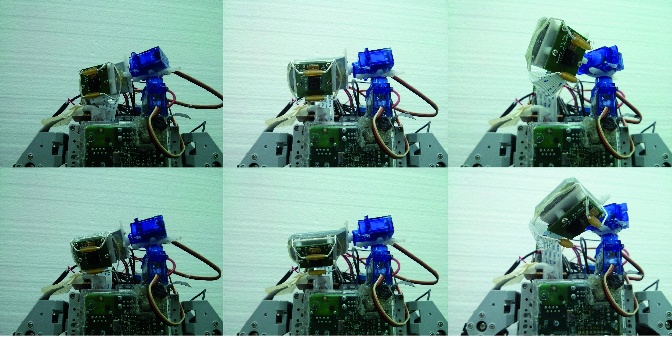
\includegraphics[scale=0.5]{imagenes/Pantallazo.png}
\caption{Posiciones de la cámara  }
\end{figure}

Estos motores se controlan desde la Arbotix usando la librería HServo. Esta librería solo puede ser usada para los motores conectados en los puertos Hobby A y B (pines 12 y 13) (ver la figura ~\ref{fig:puertosHobby}). Brinda la ventaja de un control más preciso, evitando que los motores tengan una vibración ya que los pulsos son generados por temporizadores de hardware. 

